\section{The Accuracy--Cost Frontier}\label{sec:frontier}

Figure~\ref{fig:frontier} places every method we run on the two main benchmarks by its training payload per sample and its score. On both, the envelope consists of foundation-encoder points only (\frVbNParetoFound{} of \frVbNPareto{} points on VertiBench, \frMilkNParetoFound{} of \frMilkNPareto{} on MILK10k); which regime lies on it depends on the budget and the domain. We claim a default, not strict domination: on party compute alone, a frozen ImageNet ResNet-50 (8 GFLOPs per image, 80.9\,\%) is cheaper than every foundation encoder we test, an exception that does not change the default.

\begin{figure}[t]
\centering\IfFileExists{gen/fig_frontier.pdf}{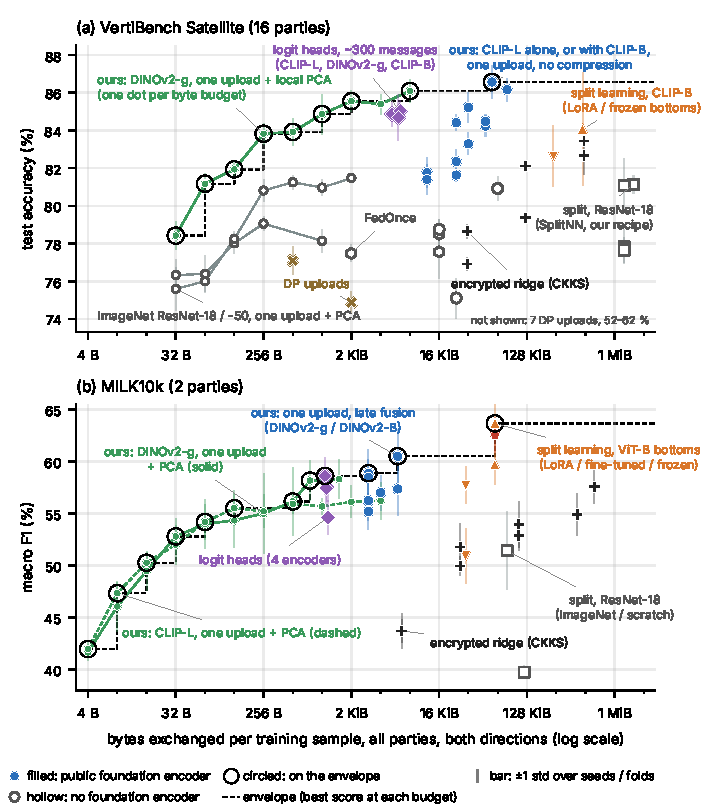
\includegraphics[width=0.92\linewidth]{gen/fig_frontier.pdf}}{\fbox{\parbox{0.9\linewidth}{\centering fig\_frontier pending}}}
\caption{The accuracy--communication frontier on VertiBench Satellite (left) and MILK10k (right). Horizontal axis: bytes exchanged per training sample over a training run, all parties and both directions (for the encrypted heads, the encrypted upload only). Filled markers use a foundation encoder, hollow ones do not; bars: std over seeds or folds; circled: envelope. VertiBench PCA points are selected on validation at each budget; seven DP points (\dpFullOne--\dpStEight\,\%) lie below the axis.}\label{fig:frontier}
\end{figure}

\subsection{VertiBench: one compressed upload is the knee}\label{sec:frontier-vb}\phantomsection\label{sec:exp-main}

\begin{table}[t]
\caption{VertiBench Satellite (16 parties, official test set). Upload: training payload per sample over all parties (activations or logits up, gradients down when needed). GFLOPs: party compute per image (a training run for split learning, one forward pass otherwise). Time: minutes on one A100 (split training, FedOnce pre-training or feature extraction). Mean\,$\pm$\,std over 5 seeds unless noted; --: not recorded.}\label{tab:main}
\centering\scriptsize
\setlength{\tabcolsep}{3pt}
\begin{adjustbox}{max width=\linewidth}
\begin{tabular}{@{}lcrrrccc@{}}
\toprule
Method & Bands & Upload & GFLOPs & Time & Acc. (\%) & F1 (\%) & AUC (\%)\\
\midrule
\inputtab{gen/tab_main.tex}
\bottomrule
\end{tabular}
\end{adjustbox}
\end{table}

\paragraph{No trained or split-learning point is on the envelope.}
Our split-learning recipe matches the reproduced reference only from ImageNet weights (\splitPTAcc\,\%), and FedOnce, whose parties pre-train their own encoders, reaches \natAcc{} to \sslAllAcc\,\% (Table~\ref{tab:main}). The best non-foundation point, the reproduced SplitNN (\frVbBestNonFound\,\% for \frVbBestNonFoundBytes{} over 50 synchronised epochs), is matched by one upload of \frVbBeatNonFoundBytes{} per sample (\frVbBeatNonFoundName: \frVbBeatNonFound\,\%), with \frVbBeatNonFoundRatio{} times fewer bytes. The frozen ResNet-50 (80.9\,\% for 64\,KiB) is off the envelope too; we have not compressed its features.
% UPDATE when the ResNet-18/50 + PCA control on VertiBench is available.

\paragraph{One upload.}
Uncompressed, frozen CLIP-L reaches \vbClipAcc\,\% (32\,KiB), DINOv2-g \vbGAcc\,\% and CLIP-B \vbClipBAcc\,\%. Against a three-seed SplitNN re-run (\auSnAll\,\%), CLIP-L gains $\pairSnClipDiff$ points ($[\pairSnClipLo,\pairSnClipHi]$, $p\pairSnClipP$), CLIP-B $\pairSnClipBDiff$ ($p\pairSnClipBP$) and DINOv2-g $\pairSnGDiff$, which is not significant ($[\pairSnGLo,\pairSnGHi]$, $p\pairSnGP$); the four-logit heads give $p\pairSnLgClipP$, $p\pairSnLgGP$ and $p\pairSnLgClipBP$, and LoRA split learning $p\pairSnLoraP$. All eight leads are positive and grow without training siblings (CLIP-L: $\pairSnClipNoSibDiff$ points, $p\pairSnClipNoSibP$), but the $p$-values are uncorrected: a Holm correction leaves only LoRA and the CLIP-B four-logit head below 0.05. The compressed uploads below were not paired-tested.

\paragraph{The PCA knee.}\phantomsection\label{sec:exp-compress}
Selected on validation under a byte budget, DINOv2-g uploads compressed by each party reach \selTwoAcc\,\% at \selTwoBytes{} per sample (all 16 parties), \selTwokAcc\,\% at \selTwokBytes{} (\selTwokCfg) and \selFullAcc\,\% at \selFullBytes, against \fullAcc\,\% uncompressed at 48\,KiB: on few labels, compression also regularises (App.~\ref{app:pca}). Beyond \selTwokBytes, four times more bytes buy half a point, and the most accurate point, two encoders side by side, reaches \frVbBest\,\% at \frVbBestBytes. This standard compression has limits: incompatible per-party bases break a head that averages the parties' vectors (\poolGMean{} to \poolGPcaMean\,\%; Sec.~\ref{sec:frontier-enc}), and on MILK10k PCA slightly lowers macro F1 (\mrGPca{} vs.\ \mrGCat\,\%, DINOv2-g).

\paragraph{Rounds and adaptation do not pay here.}
The four-logit heads reach \lgClipAcc\,\% (CLIP-L), \lgGAcc\,\% (DINOv2-g) and \lgClipBAcc\,\% (CLIP-B) for \lgClipUp--\lgGUp{} over about \lgClipEp{} synchronised epochs, below the \selTwokBytes{} upload; their interest is exposure (Sec.~\ref{sec:server}). Split learning with CLIP-B bottoms reaches \vbSplitLoraAcc\,\% with LoRA (\vbSplitLoraN{} seeds, \vbSplitLoraUp) and \vbSplitFrozenAcc\,\% frozen, against \vbClipBAcc\,\% for one upload of the same encoder: on VertiBench the most accurate points are frozen.

\paragraph{Party compute.}
Without backpropagation, a party computes one cacheable forward pass per image, which is not minimal compute: DINOv2-g costs \vbGGF{} GFLOPs per image, more than the \rEighteenTrainGF{} of training the SplitNN bottom, CLIP-B \vbClipBGF{} and ResNet-50 8. Encoding all images takes \vbGMin{} minutes with DINOv2-g and \vbClipBMin{} with CLIP-B on one A100, against \reproMin{} per SplitNN run\IfFileExists{gen/fig_frontier_axes.pdf}{ (frontier along compute, rounds and exposure: Fig.~\ref{fig:frontier-axes})}{}.

\subsection{MILK10k: the price of freezing}\label{sec:frontier-milk}\phantomsection\label{sec:exp-freeze}

\begin{table}[t]
\caption{The price of freezing on MILK10k (2 parties, 5 folds, class-balanced loss). Split learning trains the bottoms with the server's gradients; one-shot rows use frozen features and an MLP head (concatenation, or late fusion on features averaged over 8 rotations and flips). Upload per training sample: over 10 epochs for split learning, once for one-shot. Time: minutes per fold (one-shot: encoding, estimated).}\label{tab:freeze}
\centering\scriptsize
\setlength{\tabcolsep}{3pt}
\begin{adjustbox}{max width=\linewidth}
\begin{tabular}{@{}llrrrccc@{}}
\toprule
Party models & Training & Trainable & Upload & Time & F1 (\%) & Bal.\ acc.\ (\%) & Acc.\ (\%)\\
\midrule
\inputtab{gen/tab_freeze.tex}
\bottomrule
\end{tabular}
\end{adjustbox}
\end{table}

\paragraph{Adaptation is the accuracy end.}
A \frMilkBeatNonFoundBytes{} upload (\frMilkBeatNonFoundName) already reaches \frMilkBeatNonFound\,\% macro F1, above the best non-foundation point, ImageNet ResNet-18 split learning (\frMilkBestNonFound\,\% for \frMilkBestNonFoundBytes). The envelope continues through multi-view late fusion (\frMilkBestOneShot\,\% for \frMilkBestOneShotBytes) to DINOv2-B with LoRA (\frMilkBest\,\% for \frMilkBestBytes), whose lead is smaller than its fold standard deviation. With the same backbone and head, LoRA raises F1 from \fzdinovTwob{} to \fzdinovTwoblora\,\% (DINOv2-B) and from \fzclipbSixteen{} to \fzclipbSixteenlora\,\% (CLIP-B); full fine-tuning is no better (\fzdinovTwobft\,\%). Freezing thus costs \fzGapCb{} to \fzGapB{} points, but split learning also trains on augmented images: when the frozen parties average the features of 8 rotations and flips and the server fuses per-party heads, the gap shrinks to \fzGapViewsCb--\fzGapViewsB{} points (late fusion beats concatenation on all folds, as expected from modality competition~\cite{wang2020makes,peng2022balanced}; App.~\ref{app:milk}). Under one split-learning recipe, LoRA beats frozen bottoms on all folds ($\srGapB\pm\srGapSdB$ points for DINOv2-B, $\srGapCb\pm\srGapSdCb$ for CLIP-B), but frozen CLIP-B bottoms then shift F1 by $\srVsHeadCb$ points relative to the one-shot head, so part of that gain reflects a weak baseline. These points require every party to backpropagate on a GPU and stay online, exchanging \fzUpdinovTwoblora{} per sample instead of 3\,KiB once. We have not run the four-logit head or DP on MILK10k.
% UPDATE when the MILK10k four-logit and PCA-grid runs are available.

\paragraph{When to adapt.}
Adaptation buys several F1 points on dermatology images and nothing on Sentinel-2 composites, which we attribute to their distance from web-scale pre-training data, a hypothesis two benchmarks cannot establish. Domain encoders do not close the gap: SSL4EO-S12 stays below CLIP-L on VertiBench (Table~\ref{tab:main}), BiomedCLIP and MONET below DINOv2-g on MILK10k (App.~\ref{app:milk}).

\subsection{Encoder choice and missing parties}\label{sec:frontier-enc}
Pre-trained ViTs lie within a few points of each other on VertiBench, a randomly initialised ViT-B reaches 75.1\,\% (App.~\ref{app:vb}), and small encoders (DINOv2-S: \vbDinoSAcc\,\%, \vbDinoSGF{} GFLOPs) suit parties without accelerators. With 12 of 16 parties missing at inference, a concatenation head falls to \missZeroTwelveZ\,\% if missing uploads are zeroed and \missZeroTwelveM\,\% with mean imputation, whereas a head that normalises and averages the vectors of the parties present keeps \poolMissTwelve\,\% (\poolMissFifteen\,\% with one party); it needs a shared feature space, which per-party PCA and distinct modalities remove.
